\documentclass[a4paper,11pt,oneside]{report}

\usepackage{listings}
\usepackage{amsmath}
\usepackage[mathletters]{ucs}
\usepackage[utf8x]{inputenc}
\usepackage{graphicx}
\usepackage{footmisc}
\usepackage{hyperref} 
\usepackage[usenames,dvipsnames]{color}
\hypersetup{urlcolor=OliveGreen,citecolor=OliveGreen,linkcolor=BrickRed,colorlinks=true}
\setcounter{tocdepth}{1}
\usepackage[super]{natbib}
\renewcommand{\familydefault}{\sfdefault}
\renewcommand{\thefootnote}{\alph{footnote}} 

\usepackage{array}
% This is needed because raggedright in table elements redefines \\:
\newcommand{\PreserveBackslash}[1]{\let\temp=\\#1\let\\=\temp}
\let\PBS=\PreserveBackslash

\usepackage{parskip}

\lstset{
   basicstyle=\footnotesize\ttfamily,
   identifierstyle=,
   keywordstyle=,
   xleftmargin=8mm,
%   framesep=10mm,
   framextopmargin=1mm,
   framexbottommargin=1mm,
   frame=l,
   numbers=none,
   showspaces=false,
   columns=flexible,
}

\lstnewenvironment{bash}
{\lstset{language=bash}}
{}

\lstnewenvironment{lsturl}
{\lstset{language=bash,numbers=none}}
{}

\begin{document}
\bibliographystyle{moa}
\title{Moa}
\author{Mark Fiers}
\date{#DATE#}

%create a title page
\begin{titlepage}
\center{\includegraphics[width=0.6\textwidth]{images/moa_logo_medium.png}}
\center{\includegraphics[width=0.6\textwidth]{images/pfr_logo.jpg}}
\vfill
\center{\Huge Moa \normalsize}
\center{ #MOAVERSION# }
\vfill
\vfill
\center{author: Mark Fiers}
\center{date: #DATE#}
\center{\tiny git: #GITBRANCH# #GITVERSION# \normalsize}
\end{titlepage}
\tableofcontents
%end of the title page

\chapter{Introduction\label{ch:introduction}}
\chapter{Introduction}

Kea is a simple, but powerful, script automation system. It is useful
for automating small scripts that need to be executed regularly, or
need to be repeated many times, for example for a set of different
input files.

For example, a BLAST analysis \citep{Altschul1990}, you could perform
a single analysis using the following command:

\begin{lstlisting}
blastall -i seq1.fasta -o blast1.out -p blastn -d nr
\end{lstlisting}

Now suppose you want to repeat this for a set of sequences. This is,
again, not very difficult using the following bash script:

\begin{lstlisting}
for in in /data/seq/*.fasta; do
  blastall -i $in -p blastn -d nr \
      -o `basename $in .fasta`.out
done
\end{lstlisting}

But what if you would like to repeat this weekly, for several data
sets, against a few databases, but only for those sequences that have
changed? Furthermore, the sequences come from different sources with
different naming strategies and you would like uniformly named output?
It can all be done using bash, or any other scripting language, but,
you will write a lot of boilerplate code. Kea can help you.

\section{Kea}

To get started, we'll set up a job with Kea executing the sample from
above. But first, lets introduce Kea basics.

\begin{figure}[h]
  \begin{center}
    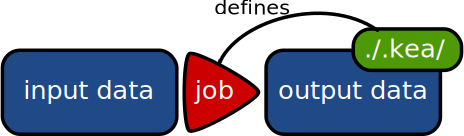
\includegraphics[width=0.6\textwidth]{kea_intro_1.pdf}
  \end{center}
  \caption{Basic structure of a Kea job; A job is usually defined in
    the directory where the results end up.}
  \label{f_intro_1}
\end{figure}

Kea automates the execution of (small) scripts. Each script automated
by Kea is called a Kea job. The author proposes that you store in and
output files in separate directories with the Kea jobs described in
the directories where the output files are stored. Kea itself does not
make such a demand. Kea assumes that for each job the input
and output files are stored in separate directories. A Kea Job is
typically linked to the directory where the results of the job are
stored (see \ref{f_intro_1}. A Kea job is linked to a directory by
storing the configuration in a sub-directory called \lstinline{./.kea}

Linking a Kea job to a single directory, allowing only one job per
directory is a conscious design decision. It keeps jobs organized and
makes execution and re-execution of jobs simple (as you will see
later), without putting actual limits on what you can do.

Back to our earlier example. Suppose that the original sequences live
in a directory called \lstinline{/data/seq/} and the blast results are
to end up in \lstinline{/data/blast}. The first step would be to
create and move to the target directory\footnote{I find it difficult
  to estimate the right level of detail. Although I do not expect that
  anybody able to operate Kea really needs to be told how to use
  \lstinline!cd! or \lstinline{mkdir}, but I prefer to add to much
  details rather than too little}:

\begin{lstlisting}
mkdir /data/seq
cd /data/seq
\end{lstlisting}

Secondly, create a basic kea configuration using the following
command:

\begin{lstlisting}
kea new
\end{lstlisting}

This command creates a \lstinline!.kea! sub-directory (if it doesn't
exists) and copies a basic configuration file. This configuration file
is named \lstinline!./.kea/local.conf! and controls what exactly your
job will do. Once you open it in an text editor it looks like a normal
configuration file. It is divided up in sections that each have a
number of options. Currently you can ignore most of these options. To
get our blast running, there are two sections that need some
work. First we'll define the BLAST input in, suprisingly, the
\lstinline![INPUT]! section. If you using the directories suggested
earlier, set the \lstinline![INPUT]! section to:

\begin{lstlisting}
[INPUT]
glob=/data/seq/*.fasta
\end{lstlisting}

or, depending on where you're target directory is, and thus where you
have defined your current Kea job, you could define the input section
using relative locations:

\begin{lstlisting}
[INPUT]
glob=../seq/*.fasta
\end{lstlisting}

Using relative directory locations makes it easy to shuffle your jobs
around, as long as their location relative to each other doesn't change.

The second part of the configuration that needs editting is the
\lstinline![ACTION]! section. This section defines what needs to be
done. For this example, change it to:

\begin{lstlisting}
[ACTION]
main = blastall -i $inputFile -d nr -p blastn -o $baseName.out
\end{lstlisting}

This defines one item (main) in the action section. It is possible to
have scripts of multiple lines, for example, if you would like to
print some extra information, you could extend your configuration like
this:

\begin{lstlisting}
[ACTION]
main =
  echo "start with $inputFile"  
  time blastall -i $inputFile -d nr -p blastn -o $baseName.out
  echo "$inputFile has finished"
\end{lstlisting}

To make sure the configuration file is parsed properly, it is
important that there is a space in front of each line of the
script. The main item is extended until there is a character in the
first column (where it is assumed that a new item starts). This allows
longer scripts.

The attentive reader might have noticed that there are two, as of yet,
unexplained variables in the scripts. These are provided by Kea.

In general terms, you give Kea a script and define some
conditions. Kea subsequently executes the script as many times as
necessary. All communication between Kea and the script go through
environment variables.

In the example above, Kea determines how many \lstinline{*.fasta}
files there are in \lstinline{/data/seq} and iteratively executes the
script once for each of those inputfiles with the full path of each
ddinput file stored in the \lstinline{$inputFile} environment variable. 
%$

asdf

% LocalWords:  conf

\chapter{Installation\label{ch:installation}}
\chapter{Installation}

.. to be written ..


\section{Getting the code}

\section{Install python libs}

\section{Set up a basic configuration}

\section{Test}

\chapter{Using Moa\label{ch:using}}
\input{using}
\chapter{Using GBrowse\label{ch:gbrowse}}
\input{gbrowse}
\chapter{Couchdb\label{ch:couchdb}}
\input{couchdb}
\chapter{Extending Moa\label{ch:extending}}
\input{extending}
\appendix
\chapter{Template reference\label{ch:templateref}}
\input{reference}

\addcontentsline{toc}{chapter}{Bibliography}
\bibliography{manual}
\end{document}
